
% EXPERIMENTO 4
\subsection{Experimento 4: sustitución de la media aritmética por funciones OWA en la construcción de los conjuntos difusos en el algoritmo 1}
Para todos los experimentos que se disponen en este capítulo, tomaremos la determinación de sustituir la media aritmética que se utiliza en la construcción de los conjuntos difusos (def. \ref{def:mediasmonoumbral} y \ref{def:conjuntodifusomonoumbral}) por una función OWA de tipo `la mayoría de' (def. \ref{def:owa}). Para ello se debe destacar el hecho de que habrá que introducir todos los datos en forma normalizada (con valores en el intervalo $[0,1]$).

En concreto se utilizarán dos variantes de funciones OWA. La primera de ellas, OWA (1), crea los pesos según la ecuación \ref{eq:pesosowamayoria} habiendo ordenado el vector en función del histograma. En el segundo caso, OWA (2), crearemos los pesos de igual manera, pero en el momento de aplicarlos los multiplicaremos por la función $h(q)$ que les corresponda.

\subsubsection{Explicación del experimento}
En este primer experimento se sustituirá la media aritmética en la creación de los conjuntos difusos en el algoritmo 1. Se hará con las dos opciones de OWA presentadas. Se conoce de antemano que debido a la necesidad del cálculo de los pesos, el tiempo de computación crecerá bastante frente a la versión original.


\subsubsection{Resultados}

En las tablas \ref{tab:resultexp4dombi} y \ref{tab:resultexp4ruido} se muestran los resultados obtenidos para todas las imágenes que se toman como muestra. Se ha de destacar que este experimento, al igual que todos, se ha llevado a cabo con un conjunto de casi 30 imágenes de las que se presentan las de resultados más significativos. 

Se puede observar claramente que los resultados obtenidos son extremadamente alejados de la realidad. Se crean únicamente umbrales que no permiten llevar a cabo ninguna segmentación de forma adecuada por lo que se omite la presentación de los resultados gráficos así como de los errores para este experimento.


\begin{table}
\centering
\begin{tabular}{c||c|c|c} 
\multicolumn{4}{c}{}\\
Silla                                &\bb Media&\bb OWA (1)&\bb OWA (2)\\\hline\hline
\bb Alg. 1 con $\mathbf{REF_1=1-\abs{x-y}}$         &   127 &   50  &   50  \\\hline
\bb Alg. 1 con $\mathbf{REF_1=1-\abs{x-y}^2}$       &   127 &   50  &   246 \\\hline
\bb Alg. 1 con $\mathbf{REF_1=1-\abs{x-y}^{0.5}}$   &   119 &   50  &   50  \\\hline
\bb Alg. 1 con $\mathbf{REF_1=(1-\abs{x-y})^2}$     &   127 &   50  &   50  \\\hline
\bb Alg. 1 con $\mathbf{REF_1=(1-\abs{x-y})^{0.5}}$ &   127 &   50  &   50  \\\hline
\multicolumn{4}{c}{}\\
Bloques                              &\bb Media&\bb OWA (1)&\bb OWA (2)\\\hline\hline
\bb Alg. 1 con $\mathbf{REF_1=1-\abs{x-y}}$         &   79  &   12  &   7   \\\hline
\bb Alg. 1 con $\mathbf{REF_1=1-\abs{x-y}^2}$       &   97  &   11  &   10  \\\hline
\bb Alg. 1 con $\mathbf{REF_1=1-\abs{x-y}^{0.5}}$   &   47  &   13  &   4   \\\hline
\bb Alg. 1 con $\mathbf{REF_1=(1-\abs{x-y})^2}$     &   70  &   14  &   7   \\\hline
\bb Alg. 1 con $\mathbf{REF_1=(1-\abs{x-y})^{0.5}}$ &   82  &   12  &   10  \\\hline
\multicolumn{4}{c}{}\\
Engranaje                            &\bb Media&\bb OWA (1)&\bb OWA (2)\\\hline\hline
\bb Alg. 1 con $\mathbf{REF_1=1-\abs{x-y}}$         &   104 &   7   &   4   \\\hline
\bb Alg. 1 con $\mathbf{REF_1=1-\abs{x-y}^2}$       &   104 &   13  &   4   \\\hline
\bb Alg. 1 con $\mathbf{REF_1=1-\abs{x-y}^{0.5}}$   &   84  &   4   &   1   \\\hline
\bb Alg. 1 con $\mathbf{REF_1=(1-\abs{x-y})^2}$     &   105 &   5   &   4   \\\hline
\bb Alg. 1 con $\mathbf{REF_1=(1-\abs{x-y})^{0.5}}$ &   104 &   11  &   4   \\\hline
\multicolumn{4}{c}{}\\
Letras                               &\bb Media&\bb OWA (1)&\bb OWA (2)\\\hline\hline
\bb Alg. 1 con $\mathbf{REF_1=1-\abs{x-y}}$         &   187 &   255 &   239 \\\hline
\bb Alg. 1 con $\mathbf{REF_1=1-\abs{x-y}^2}$       &   174 &   255 &   239 \\\hline
\bb Alg. 1 con $\mathbf{REF_1=1-\abs{x-y}^{0.5}}$   &   200 &   255 &   239 \\\hline
\bb Alg. 1 con $\mathbf{REF_1=(1-\abs{x-y})^2}$     &   190 &   255 &   236 \\\hline
\bb Alg. 1 con $\mathbf{REF_1=(1-\abs{x-y})^{0.5}}$ &   186 &   255 &   255 \\\hline
\multicolumn{4}{c}{}\\
Sombra                               &\bb Media&\bb OWA (1)&\bb OWA (2)\\\hline\hline
\bb Alg. 1 con $\mathbf{REF_1=1-\abs{x-y}}$         &   123 &   255 &   231 \\\hline
\bb Alg. 1 con $\mathbf{REF_1=1-\abs{x-y}^2}$       &   126 &   255 &   255 \\\hline
\bb Alg. 1 con $\mathbf{REF_1=1-\abs{x-y}^{0.5}}$   &   121 &   46  &   85  \\\hline
\bb Alg. 1 con $\mathbf{REF_1=(1-\abs{x-y})^2}$     &   123 &   255 &   202 \\\hline
\bb Alg. 1 con $\mathbf{REF_1=(1-\abs{x-y})^{0.5}}$ &   124 &   255 &   255 \\\hline
\end{tabular}
\caption{Umbrales para todas las versiones del algoritmo 1 con la aplicación de OWA.\label{tab:resultexp4dombi}}
\end{table}




\begin{table}
\centering
\begin{tabular}{c||c|c|c} 
\multicolumn{4}{c}{}\\
R. gausiano                         &\bb Media&\bb OWA (1)&\bb OWA (2)\\\hline\hline
\bb Alg. 1 con $\mathbf{REF_1=1-\abs{x-y}}$         &   131 &   50  &   0   \\\hline
\bb Alg. 1 con $\mathbf{REF_1=1-\abs{x-y}^2}$       &   131 &   12  &   0   \\\hline
\bb Alg. 1 con $\mathbf{REF_1=1-\abs{x-y}^{0.5}}$   &   132 &   56  &   0   \\\hline
\bb Alg. 1 con $\mathbf{REF_1=(1-\abs{x-y})^2}$     &   131 &   56  &   0   \\\hline
\bb Alg. 1 con $\mathbf{REF_1=(1-\abs{x-y})^{0.5}}$ &   131 &   43  &   0   \\\hline
\multicolumn{4}{c}{}\\
R. impulsivo 0,05                    &\bb Media&\bb OWA (1)&\bb OWA (2)\\\hline\hline
\bb Alg. 1 con $\mathbf{REF_1=1-\abs{x-y}}$         &   127 &   50  &   50  \\\hline
\bb Alg. 1 con $\mathbf{REF_1=1-\abs{x-y}^2}$       &   127 &   50  &   50  \\\hline
\bb Alg. 1 con $\mathbf{REF_1=1-\abs{x-y}^{0.5}}$   &   144 &   50  &   50  \\\hline
\bb Alg. 1 con $\mathbf{REF_1=(1-\abs{x-y})^2}$     &   127 &   50  &   50  \\\hline
\bb Alg. 1 con $\mathbf{REF_1=(1-\abs{x-y})^{0.5}}$ &   127 &   50  &   50  \\\hline
\multicolumn{4}{c}{}\\
R. impulsivo 0,2                     &\bb Media&\bb OWA (1)&\bb OWA (2)\\\hline\hline
\bb Alg. 1 con $\mathbf{REF_1=1-\abs{x-y}}$         &   127 &   50  &   50  \\\hline
\bb Alg. 1 con $\mathbf{REF_1=1-\abs{x-y}^2}$       &   127 &   50  &   0   \\\hline
\bb Alg. 1 con $\mathbf{REF_1=1-\abs{x-y}^{0.5}}$   &   152 &   50  &   0   \\\hline
\bb Alg. 1 con $\mathbf{REF_1=(1-\abs{x-y})^2}$     &   127 &   50  &   50  \\\hline
\bb Alg. 1 con $\mathbf{REF_1=(1-\abs{x-y})^{0.5}}$ &   127 &   50  &   0   \\\hline
\end{tabular}
\caption{Umbrales para todas las versiones del algoritmo 1 con la aplicación de OWA para imágenes con ruido.\label{tab:resultexp4ruido}}
\end{table}


% EXPERIMENTO 5
\subsection{Experimento 5: sustitución de la media aritmética por funciones OWA en la construcción de los conjuntos difusos para el algoritmo 2 con función penalti}

\subsubsection{Explicación del experimento}
Para este experimento se sustituirá la media aritmética en la creación del numerador necesario en el algoritmo 2. De nuevo, se hará con las dos opciones de OWA presentadas. De forma recurrente, también, se tiene en cuenta que el tiempo de cómputo subirá de forma extraordinaria, más aun si recordamos que este algoritmo inicialmente hacía pocos cálculos y, por tanto, utiliza poco tiempo.

\subsubsection{Resultados}

Si se estudian las tablas \ref{tab:resultexp5dombi} y \ref{tab:resultexp5ruido} se encontrarán de nuevo unos resultados decepcionantes para la umbralización llevada a cabo. Excepto en casos concretos (todos ellos dependientes de $\varphi_1=x^{0,5} \text{ y }\varphi_2=x$).

Se puede observar que claramente los resultados obtenidos son extremadamente alejados de la realidad. Se crean únicamente umbrales que no permiten llevar a cabo ninguna segmentación de forma adecuada por lo que se omite, de nuevo, la presentación de los resultados gráficos así como de los errores en este experimento.

\begin{table}
\centering
\begin{tabular}{c||c|c|c} 
\multicolumn{4}{c}{}\\
Silla                                &\bb Media&\bb OWA (1)&\bb OWA (2)\\\hline\hline
\bb Alg. 2 con $\mathbf{\varphi_1=\varphi_2=x}$     &   119 &   50  &   50  \\\hline
\bb Alg. 2 con $\mathbf{\varphi_1=x^2 \text{ y }\varphi_2=x}$   &   119 &   58  &   50  \\\hline
\bb Alg. 2 con $\mathbf{\varphi_1=x^{0,5} \text{ y }\varphi_2=x}$     &   103 &   114 &   172 \\\hline
\bb Alg. 2 con $\mathbf{\varphi_1=1-\sqrt{1-x} \text{ y }\varphi_2=x}$  &   127 &   50  &   50  \\\hline
\multicolumn{4}{c}{}\\
Bloques                              &\bb Media&\bb OWA (1)&\bb OWA (2)\\\hline\hline
\bb Alg. 2 con $\mathbf{\varphi_1=\varphi_2=x}$     &   47  &   13  &   4   \\\hline
\bb Alg. 2 con $\mathbf{\varphi_1=x^2 \text{ y }\varphi_2=x}$   &   39  &   13  &   4   \\\hline
\bb Alg. 2 con $\mathbf{\varphi_1=x^{0,5} \text{ y }\varphi_2=x}$     &   30  &   11  &   65  \\\hline
\bb Alg. 2 con $\mathbf{\varphi_1=1-\sqrt{1-x} \text{ y }\varphi_2=x}$  &   79  &   12  &   7   \\\hline
\multicolumn{4}{c}{}\\
Engranaje                            &\bb Media&\bb OWA (1)&\bb OWA (2)\\\hline\hline
\bb Alg. 2 con $\mathbf{\varphi_1=\varphi_2=x}$     &   84  &   4   &   1   \\\hline
\bb Alg. 2 con $\mathbf{\varphi_1=x^2 \text{ y }\varphi_2=x}$   &   78  &   4   &   0   \\\hline
\bb Alg. 2 con $\mathbf{\varphi_1=x^{0,5} \text{ y }\varphi_2=x}$     &   147 &   89  &   193 \\\hline
\bb Alg. 2 con $\mathbf{\varphi_1=1-\sqrt{1-x} \text{ y }\varphi_2=x}$  &   104 &   7   &   4   \\\hline
\multicolumn{4}{c}{}\\
Letras                               &\bb Media&\bb OWA (1)&\bb OWA (2)\\\hline\hline
\bb Alg. 2 con $\mathbf{\varphi_1=\varphi_2=x}$     &   121 &   46  &   85  \\\hline
\bb Alg. 2 con $\mathbf{\varphi_1=x^2 \text{ y }\varphi_2=x}$   &   121 &   54  &   86  \\\hline
\bb Alg. 2 con $\mathbf{\varphi_1=x^{0,5} \text{ y }\varphi_2=x}$     &   101 &   136 &   136 \\\hline
\bb Alg. 2 con $\mathbf{\varphi_1=1-\sqrt{1-x} \text{ y }\varphi_2=x}$  &   123 &   255 &   231 \\\hline
\multicolumn{4}{c}{}\\
Sombra                               &\bb Media&\bb OWA (1)&\bb OWA (2)\\\hline\hline
\bb Alg. 2 con $\mathbf{\varphi_1=\varphi_2=x}$     &   200 &   255 &   239 \\\hline
\bb Alg. 2 con $\mathbf{\varphi_1=x^2 \text{ y }\varphi_2=x}$   &   201 &   255 &   235 \\\hline
\bb Alg. 2 con $\mathbf{\varphi_1=x^{0,5} \text{ y }\varphi_2=x}$     &   178 &   171 &   168 \\\hline
\bb Alg. 2 con $\mathbf{\varphi_1=1-\sqrt{1-x} \text{ y }\varphi_2=x}$  &   187 &   255 &   239 \\\hline
\end{tabular}
\caption{Umbrales para todas las versiones del algoritmo 2 con la aplicación de OWA.\label{tab:resultexp5dombi}}
\end{table}


\begin{table}
\centering
\begin{tabular}{c||c|c|c} 
\multicolumn{4}{c}{}\\
R. gausiano                         &\bb Media&\bb OWA (1)&\bb OWA (2)\\\hline\hline
\bb Alg. 2 con $\mathbf{\varphi_1=\varphi_2=x}$     &   132 &   56  &   0   \\\hline
\bb Alg. 2 con $\mathbf{\varphi_1=x^2 \text{ y }\varphi_2=x}$   &   132 &   59  &   0   \\\hline
\bb Alg. 2 con $\mathbf{\varphi_1=x^{0,5} \text{ y }\varphi_2=x}$     &   99  &   154 &   159 \\\hline
\bb Alg. 2 con $\mathbf{\varphi_1=1-\sqrt{1-x} \text{ y }\varphi_2=x}$  &   131 &   50  &   0   \\\hline
\multicolumn{4}{c}{}\\
R. impulsivo 0,05                    &\bb Media&\bb OWA (1)&\bb OWA (2)\\\hline\hline
\bb Alg. 2 con $\mathbf{\varphi_1=\varphi_2=x}$     &   144 &   50  &   50  \\\hline
\bb Alg. 2 con $\mathbf{\varphi_1=x^2 \text{ y }\varphi_2=x}$   &   144 &   58  &   50  \\\hline
\bb Alg. 2 con $\mathbf{\varphi_1=x^{0,5} \text{ y }\varphi_2=x}$     &   111 &   122 &   172 \\\hline
\bb Alg. 2 con $\mathbf{\varphi_1=1-\sqrt{1-x} \text{ y }\varphi_2=x}$  &   127 &   50  &   50  \\\hline
\multicolumn{4}{c}{}\\
R. impulsivo 0,2                     &\bb Media&\bb OWA (1)&\bb OWA (2)\\\hline\hline
\bb Alg. 2 con $\mathbf{\varphi_1=\varphi_2=x}$     &   152 &   50  &   0   \\\hline
\bb Alg. 2 con $\mathbf{\varphi_1=x^2 \text{ y }\varphi_2=x}$   &   160 &   50  &   0   \\\hline
\bb Alg. 2 con $\mathbf{\varphi_1=x^{0,5} \text{ y }\varphi_2=x}$     &   127 &   131 &   172 \\\hline
\bb Alg. 2 con $\mathbf{\varphi_1=1-\sqrt{1-x} \text{ y }\varphi_2=x}$  &   127 &   50  &   50  \\\hline
\end{tabular}
\caption{Umbrales para todas las versiones del algoritmo 2 con la aplicación de OWA para imágenes con ruido.\label{tab:resultexp5ruido}}
\end{table}


% EXPERIMENTO 6
\subsection{Experimento 6: sustitución de la media aritmética por funciones OWA en la construcción de los conjuntos difusos para el algoritmo 1 con función penalti}

\subsubsection{Explicación del experimento}
En este caso, debido a que este algoritmo es una modificación del primero, se volverá a usar funciones OWA para la creación de los conjuntos difusos que representen las imágenes. 

\subsubsection{Resultados}
Es curioso observar como el resultado cambia de forma radical. En la tabla \ref{tab:resultexp6} se pueden observar los umbrales que se encuentran aplicados en las imágenes recogidas en la tabla \ref{tab:resultexp6imagenes}. En cualquier caso, este resultado tiene aún un problema, pues se gasta mucho tiempo de computación para, como mucho, igualar el resultado sino no empeorarlo como sucede con algún ejemplo.
%\REV{falta calcular los errores}.

\begin{table}
\centering
\begin{tabular}{c||c|c|c} 
      &\bb Media&\bb OWA (1)&\bb OWA (2)\\\hline\hline
\bb Silla     &   136   &   50  &   50  \\\hline
\bb Bloques   &   82    &   12  &   10  \\\hline
\bb Engranaje &   102   &   7   &   4   \\\hline
\bb Letras    &   193   &   255 &   239 \\\hline
\bb Sombra    &   122   &   255 &   205 \\\hline
%\REV{revisar resultados tabla}
\end{tabular}
\caption{Umbrales para la versión agregada del algoritmo 1 con la aplicación de OWA y penalti.\label{tab:resultexp6}}
\end{table}


\begin{table}
\centering
\begin{tabular}{c|c|c}
\bb Media&\bb OWA (1)&\bb OWA (2)\\\hline\hline
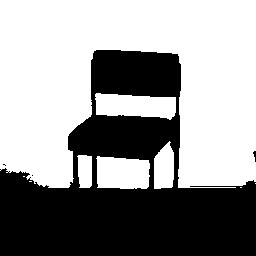
\includegraphics[width=0.15\textwidth]{img/res/e6/alg1agregadoowa1chair.jpg} &
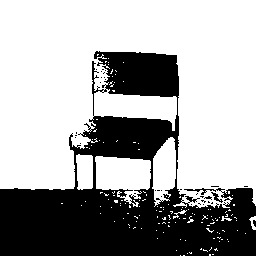
\includegraphics[width=0.15\textwidth]{img/res/e6/alg1agregadoowa2chair.jpg} &
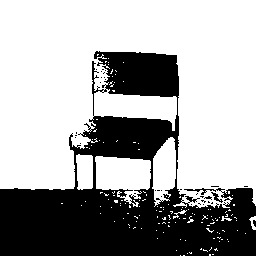
\includegraphics[width=0.15\textwidth]{img/res/e6/alg1agregadoowa3chair.jpg} \\\hline
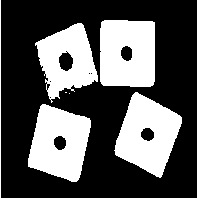
\includegraphics[width=0.15\textwidth]{img/res/e6/alg1agregadoowa1block.jpg} &
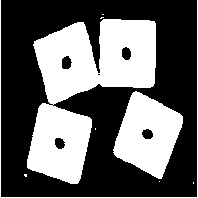
\includegraphics[width=0.15\textwidth]{img/res/e6/alg1agregadoowa2block.jpg} &
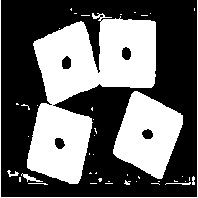
\includegraphics[width=0.15\textwidth]{img/res/e6/alg1agregadoowa3block.jpg} \\\hline
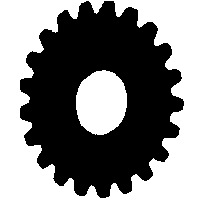
\includegraphics[width=0.15\textwidth]{img/res/e6/alg1agregadoowa102.jpg} &
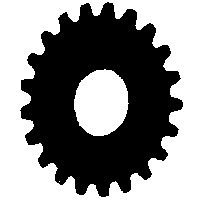
\includegraphics[width=0.15\textwidth]{img/res/e6/alg1agregadoowa202.jpg} &
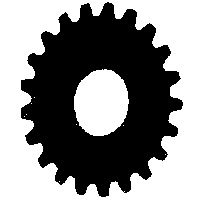
\includegraphics[width=0.15\textwidth]{img/res/e6/alg1agregadoowa302.jpg} \\\hline
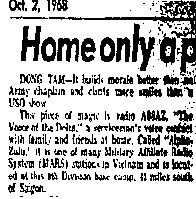
\includegraphics[width=0.15\textwidth]{img/res/e6/alg1agregadoowa109.jpg} &
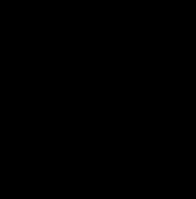
\includegraphics[width=0.15\textwidth]{img/res/e6/alg1agregadoowa209.jpg} &
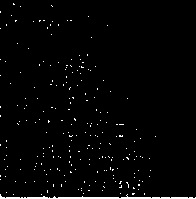
\includegraphics[width=0.15\textwidth]{img/res/e6/alg1agregadoowa309.jpg} \\\hline
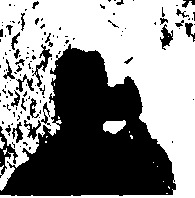
\includegraphics[width=0.15\textwidth]{img/res/e6/alg1agregadoowa107.jpg} &
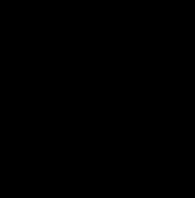
\includegraphics[width=0.15\textwidth]{img/res/e6/alg1agregadoowa207.jpg} &
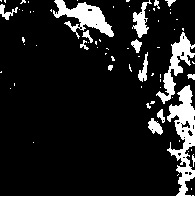
\includegraphics[width=0.15\textwidth]{img/res/e6/alg1agregadoowa307.jpg} \\\hline
\end{tabular}
\caption{Resultados gráficos para la versión agregada del algoritmo 1 con la aplicación de OWA y penalti. \label{tab:resultexp6imagenes}}
\end{table}


Se presentan, también, los resultados de aplicar el experimento sobre imágenes con ruido. Se ve que, claramente, existe una tendencia de que la segunda forma de crear el OWA haga que el umbral se dispare hacia un extremo. Aun así, y de nuevo se puede apreciar claramente con las imagenes segmentadas de la tabla \ref{tab:resultexp6imagenesruido}, la segmentación es bastante peor, sin contar el tiempo de computación extra que es necesario en relación a los algoritmos del capítulo anterior.

\begin{table}
\centering
\begin{tabular}{c||c|c|c} 
                         &\bb Media&\bb OWA (1)&\bb OWA (2)\\\hline\hline
\bb R. gausiano         &   131 &   56  &   0   \\\hline
\bb R. impulsivo 0,05   &   127 &   50  &   50  \\\hline
\bb R. impulsivo 0,2    &   136 &   50  &   50  \\\hline
\end{tabular}
\caption{Resultados gráficos para la versión agregada del algoritmo 1 con la aplicación de OWA y penalti en imágenes con ruido.\label{tab:resultexp6ruido}}
\end{table}

\begin{table}
\centering
%\resizebox*{3\textwidth}{!}{
\begin{tabular}{c|c|c} 
\multicolumn{4}{c}{}\\
\bb Media&\bb OWA (1)&\bb OWA (2)\\\hline\hline
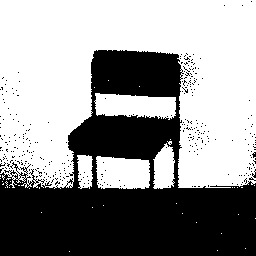
\includegraphics[width=0.15\textwidth]{img/res/e6/alg1agregadoowa1chairga.jpg} &
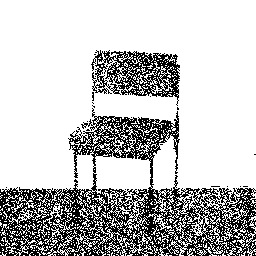
\includegraphics[width=0.15\textwidth]{img/res/e6/alg1agregadoowa2chairga.jpg} &
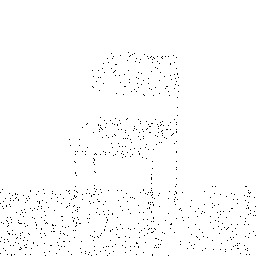
\includegraphics[width=0.15\textwidth]{img/res/e6/alg1agregadoowa3chairga.jpg} \\\hline
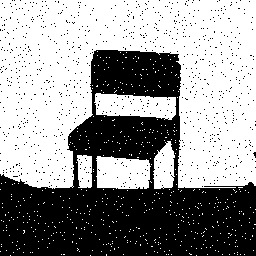
\includegraphics[width=0.15\textwidth]{img/res/e6/alg1agregadoowa1chairsp005.jpg} &
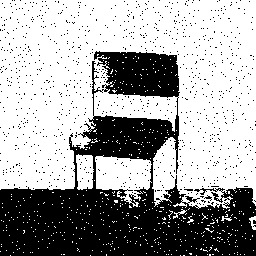
\includegraphics[width=0.15\textwidth]{img/res/e6/alg1agregadoowa2chairsp005.jpg} &
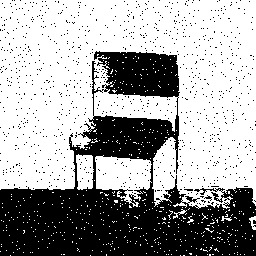
\includegraphics[width=0.15\textwidth]{img/res/e6/alg1agregadoowa3chairsp005.jpg} \\\hline
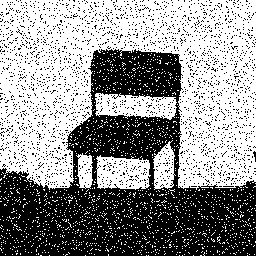
\includegraphics[width=0.15\textwidth]{img/res/e6/alg1agregadoowa1chairsp020.jpg} &
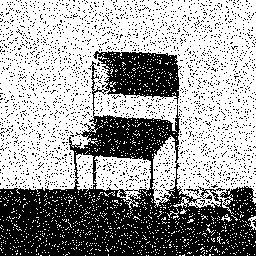
\includegraphics[width=0.15\textwidth]{img/res/e6/alg1agregadoowa2chairsp020.jpg} &
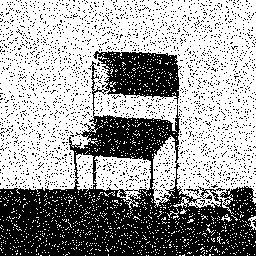
\includegraphics[width=0.15\textwidth]{img/res/e6/alg1agregadoowa3chairsp020.jpg} \\\hline
\end{tabular}
\caption{Resultados gráficos para la versión agregada del algoritmo 1 con la aplicación de OWA y penalti en imágenes con ruido.\label{tab:resultexp6imagenesruido}}
\end{table}


% EXPERIMENTO 7
\subsection{Experimento 7: sustitución de la media aritmética por funciones OWA en la construcción de los conjutos difusos para el algoritmo del umbral óptimo por similitud}
\subsubsection{Explicación del experimento}
En este caso, se cambiará la media aritmética que se encuentra en la creación del conjunto $H$ que se utiliza para conocer la similitud de las imágenes. Se mantendrá esta configuración durante todo el experimento. Únicamente cambiará la media por una función OWA que se encuentra en la creación de los conjuntos difusos que se comparan contra $H$.
\REV{Este párrafo no tiene sentido.}

Se distinguirán dos casos, por medio de las dos funciones OWA que se han explicado. Aquel que acoge a la OWA (1) es el Alg. 3 (a) y el que multiplica por el histograma será el Alg. 3 (b).
\REV{Este párrafo no tiene sentido.}

\subsubsection{Resultados}
De nuevo se vuelve a observar que no se dan buenos resultados para aquellas opciones que siguen teniendo la construcción del conjunto $Q_t$ por medio de OWA. En cambio, se observa un cambio muy interesante, ya que parece que la versión que se utiliza con la media aritmética pero con OWA para crear el conjunto $H$ obtiene grandes resultados, para el caso en el cual no se multiplica por el histograma (Alg 3 (a)). Tampoco se desdiñen los resultados obtenidos con e OWA (2), la versión (b), aunque no son tan buenos.
%\REV{errores}
\begin{table}
\centering
\begin{tabular}{c||c|c|c}
Silla                                &\bb Media&\bb OWA (1)&\bb OWA (2)\\\hline\hline
\bb Alg. 3 (a)  &   119 &   50  &   50  \\\hline
                            
\bb Alg. 3 (b)  &   103 &   114 &   172 \\\hline
\multicolumn{4}{c}{}\\
Bloques                              &\bb Media&\bb OWA (1)&\bb OWA (2)\\\hline\hline
\bb Alg. 3 (a)     &   47  &   13  &   4   \\\hline
                            
\bb Alg. 3 (b)     &   30  &   11  &   65  \\\hline
\multicolumn{4}{c}{}\\
Engranaje                            &\bb Media&\bb OWA (1)&\bb OWA (2)\\\hline\hline
\bb Alg. 3 (a)  &   84  &   4   &   1   \\\hline
                            
\bb Alg. 3 (b)  &   147 &   89  &   193 \\\hline
\multicolumn{4}{c}{}\\
Letras                               &\bb Media&\bb OWA (1)&\bb OWA (2)\\\hline\hline
\bb Alg. 3 (a)  &   200 &   255 &   236 \\\hline
                            
\bb Alg. 3 (b)  &   178 &   171 &   168 \\\hline
\multicolumn{4}{c}{}\\
Sombra                               &\bb Media&\bb OWA (1)&\bb OWA (2)\\\hline\hline
\bb Alg. 3 (a)  &   121 &   255 &   85  \\\hline
                            
\bb Alg. 3 (b)  &   101 &   136 &   136 \\\hline
\end{tabular}
\caption{Umbrales para cada imagen con el algoritmo 3 a través la aplicación de OWA.\label{tab:resultexp7}}
\end{table}

\begin{table}
\centering
%\resizebox*{3\textwidth}{!}{
\begin{tabular}{c||c|c|c} 
\multicolumn{4}{c}{}\\
Silla                                &\bb Media&\bb OWA (1)&\bb OWA (2)\\\hline\hline
\bb Alg. 3 (a)  &  
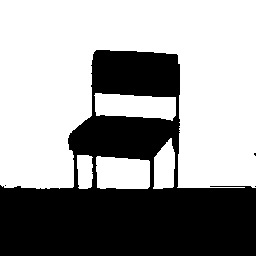
\includegraphics[width=0.12\textwidth]{img/res/e7/alg3aowa1chair.jpg} &
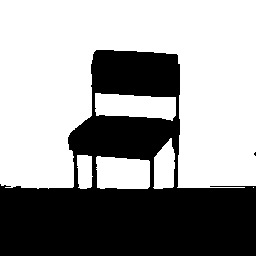
\includegraphics[width=0.12\textwidth]{img/res/e7/alg3aowa2chair.jpg} &
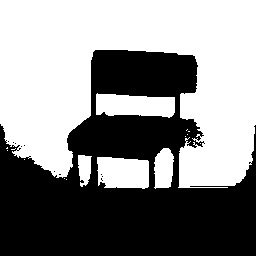
\includegraphics[width=0.12\textwidth]{img/res/e7/alg3aowa3chair.jpg} \\
\bb Alg. 3 (b)  &   
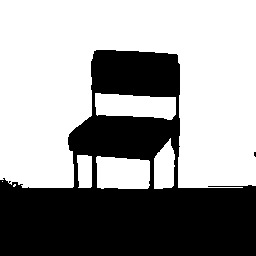
\includegraphics[width=0.12\textwidth]{img/res/e7/alg3bowa1chair.jpg} &
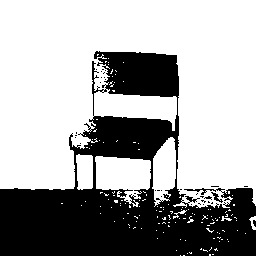
\includegraphics[width=0.12\textwidth]{img/res/e7/alg3bowa2chair.jpg} &
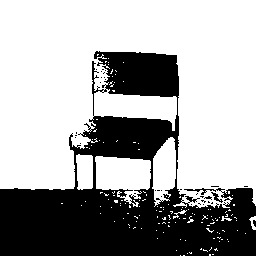
\includegraphics[width=0.12\textwidth]{img/res/e7/alg3bowa3chair.jpg} \\\hline
\multicolumn{4}{c}{}\\
Bloques                              &\bb Media&\bb OWA (1)&\bb OWA (2)\\\hline\hline
\bb Alg. 3 (a)  &  
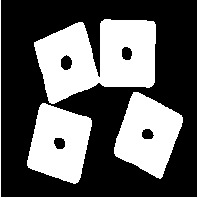
\includegraphics[width=0.12\textwidth]{img/res/e7/alg3aowa1block.jpg} &
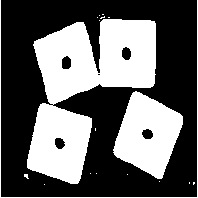
\includegraphics[width=0.12\textwidth]{img/res/e7/alg3aowa2block.jpg} &
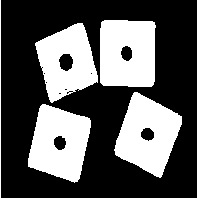
\includegraphics[width=0.12\textwidth]{img/res/e7/alg3aowa3block.jpg} \\
\bb Alg. 3 (b)  &   
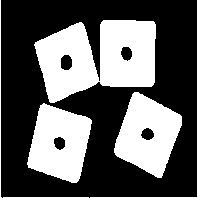
\includegraphics[width=0.12\textwidth]{img/res/e7/alg3bowa1block.jpg} &
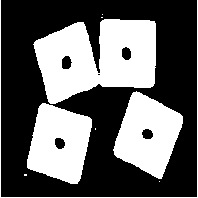
\includegraphics[width=0.12\textwidth]{img/res/e7/alg3bowa2block.jpg} &
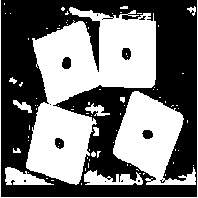
\includegraphics[width=0.12\textwidth]{img/res/e7/alg3bowa3block.jpg} \\\hline
\multicolumn{4}{c}{}\\
Engranaje                            &\bb Media&\bb OWA (1)&\bb OWA (2)\\\hline\hline
\bb Alg. 3 (a)  &  
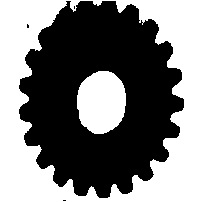
\includegraphics[width=0.12\textwidth]{img/res/e7/alg3aowa102.jpg} &
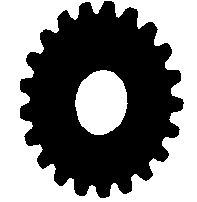
\includegraphics[width=0.12\textwidth]{img/res/e7/alg3aowa202.jpg} &
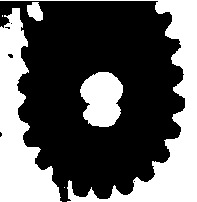
\includegraphics[width=0.12\textwidth]{img/res/e7/alg3aowa302.jpg} \\
\bb Alg. 3 (b)  &   
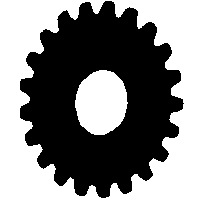
\includegraphics[width=0.12\textwidth]{img/res/e7/alg3bowa102.jpg} &
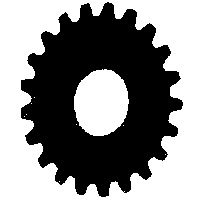
\includegraphics[width=0.12\textwidth]{img/res/e7/alg3bowa202.jpg} &
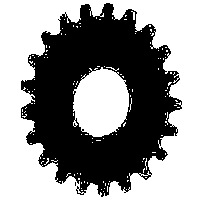
\includegraphics[width=0.12\textwidth]{img/res/e7/alg3bowa302.jpg} \\\hline
\multicolumn{4}{c}{}\\
Letras                               &\bb Media&\bb OWA (1)&\bb OWA (2)\\\hline\hline
\bb Alg. 3 (a)  &  
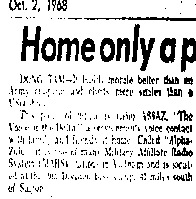
\includegraphics[width=0.12\textwidth]{img/res/e7/alg3aowa109.jpg} &
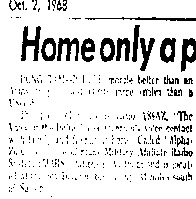
\includegraphics[width=0.12\textwidth]{img/res/e7/alg3aowa209.jpg} &
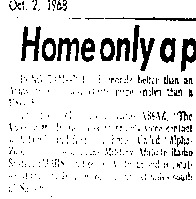
\includegraphics[width=0.12\textwidth]{img/res/e7/alg3aowa309.jpg} \\
\bb Alg. 3 (b)  &   
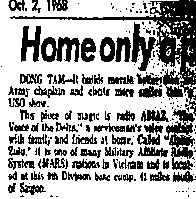
\includegraphics[width=0.12\textwidth]{img/res/e7/alg3bowa109.jpg} &
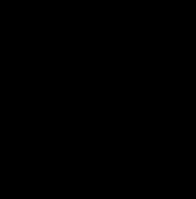
\includegraphics[width=0.12\textwidth]{img/res/e7/alg3bowa209.jpg} &
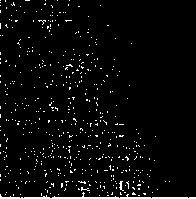
\includegraphics[width=0.12\textwidth]{img/res/e7/alg3bowa309.jpg} \\\hline
\multicolumn{4}{c}{}\\
Sombra                               &\bb Media&\bb OWA (1)&\bb OWA (2)\\\hline\hline
\bb Alg. 3 (a)  &  
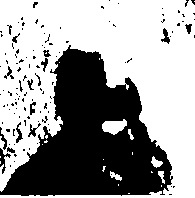
\includegraphics[width=0.12\textwidth]{img/res/e7/alg3aowa107.jpg} &
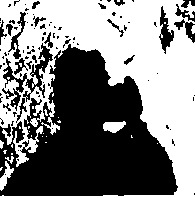
\includegraphics[width=0.12\textwidth]{img/res/e7/alg3aowa207.jpg} &
\includegraphics[width=0.12\textwidth]{img/res/e7/alg3aowa307.jpg} \\
\bb Alg. 3 (b)  &   
\includegraphics[width=0.12\textwidth]{img/res/e7/alg3bowa107.jpg} &
\includegraphics[width=0.12\textwidth]{img/res/e7/alg3bowa207.jpg} &
\includegraphics[width=0.12\textwidth]{img/res/e7/alg3bowa307.jpg} \\\hline
\end{tabular}
\caption{Resultados gráficos para el algoritmo 3 con la aplicación de OWA.\label{tab:resultexp7imagenes}}
\end{table}

En el caso de las imágenes con ruido, la tendencia es exactamente la misma. Como ha ocurrido en todos los experimentos, no se diluye el ruido ya que con una umbralización este no puede desaparecer. Esto se ve muy claro en el ruido impulsivo. Se solucionaría con la apliación previa de un filtro.

\begin{table}
\centering
\begin{tabular}{c||c|c|c}
R. gausiano                         &\bb Media&\bb OWA (1)&\bb OWA (2)\\\hline\hline
\bb Alg. 3 (a)  &   132 &   56  &   0   \\\hline
                            
\bb Alg. 3 (b)  &   99  &   154 &   159 \\\hline
\multicolumn{4}{c}{}\\
R. impulsivo 0,05                    &\bb Media&\bb OWA (1)&\bb OWA (2)\\\hline\hline
\bb Alg. 3 (a)  &   144 &   50  &   50  \\\hline
                            
\bb Alg. 3 (b)  &   111 &   122 &   172 \\\hline
\multicolumn{4}{c}{}\\
R. impulsivo 0,2                     &\bb Media&\bb OWA (1)&\bb OWA (2)\\\hline\hline
\bb Alg. 3 (a)     &   152 &   50  &   0   \\\hline
                            
\bb Alg. 3 (b)     &   127 &   131 &   172 \\\hline
\end{tabular}
\caption{Umbrales para cada imagen con el algoritmo 3 a través la aplicación de OWA en imágenes con ruido.\label{tab:resultexp7ruido}}
\end{table}

\begin{table}
\centering
\begin{tabular}{c||c|c|c} 
\multicolumn{4}{c}{}\\
R. gausiano                                 &\bb Media&\bb OWA (1)&\bb OWA (2)\\\hline\hline
\bb Alg. 3 (a)  &  
\includegraphics[width=0.12\textwidth]{img/res/e7/alg3aowa1chairga.jpg} &
\includegraphics[width=0.12\textwidth]{img/res/e7/alg3aowa2chairga.jpg} &
\includegraphics[width=0.12\textwidth]{img/res/e7/alg3aowa3chairga.jpg} \\
\bb Alg. 3 (b)  &   
\includegraphics[width=0.12\textwidth]{img/res/e7/alg3bowa1chairga.jpg} &
\includegraphics[width=0.12\textwidth]{img/res/e7/alg3bowa2chairga.jpg} &
\includegraphics[width=0.12\textwidth]{img/res/e7/alg3bowa3chairga.jpg} \\\hline
\multicolumn{4}{c}{}\\
R. impulsivo 0,05                             &\bb Media&\bb OWA (1)&\bb OWA (2)\\\hline\hline 
\bb Alg. 3 (a)  &  
\includegraphics[width=0.12\textwidth]{img/res/e7/alg3aowa1chairsp005.jpg} &
\includegraphics[width=0.12\textwidth]{img/res/e7/alg3aowa2chairsp005.jpg} &
\includegraphics[width=0.12\textwidth]{img/res/e7/alg3aowa3chairsp005.jpg} \\
\bb Alg. 3 (b)  &   
\includegraphics[width=0.12\textwidth]{img/res/e7/alg3bowa1chairsp005.jpg} &
\includegraphics[width=0.12\textwidth]{img/res/e7/alg3bowa2chairsp005.jpg} &
\includegraphics[width=0.12\textwidth]{img/res/e7/alg3bowa3chairsp005.jpg} \\\hline
\multicolumn{4}{c}{}\\
R. impulsivo 0,2                        &\bb Media&\bb OWA (1)&\bb OWA (2)\\\hline\hline
\bb Alg. 3 (a)  &  
\includegraphics[width=0.12\textwidth]{img/res/e7/alg3aowa1chairsp020.jpg} &
\includegraphics[width=0.12\textwidth]{img/res/e7/alg3aowa2chairsp020.jpg} &
\includegraphics[width=0.12\textwidth]{img/res/e7/alg3aowa3chairsp020.jpg} \\
\bb Alg. 3 (b)  &   
\includegraphics[width=0.12\textwidth]{img/res/e7/alg3bowa1chairsp020.jpg} &
\includegraphics[width=0.12\textwidth]{img/res/e7/alg3bowa2chairsp020.jpg} &
\includegraphics[width=0.12\textwidth]{img/res/e7/alg3bowa3chairsp020.jpg} \\\hline
\end{tabular}
\caption{Resultados gráficos para el algoritmo 3 con la aplicación de OWA en imágenes con ruido.\label{tab:resultexp7imagenesruido}}
\end{table}

